%--------------------------------------------------------------
% tesi.tex 
%--------------------------------------------------------------
% Corso di Laurea in Informatica 
% http://if.dsi.unifi.it/
% @Facolt\`a di Scienze Matematiche, Fisiche e Naturali
% @Universit\`a degli Studi di Firenze
%--------------------------------------------------------------
% - template for the main file of Informatica@Unifi Thesis 
% - based on Classic Thesis Style Copyright (C) 2008 
%   Andr\'e Miede http://www.miede.de   
%--------------------------------------------------------------

\documentclass[twoside,openright,titlepage,fleqn,
,	headinclude,12pt,a4paper,BCOR5mm,footinclude,table]{scrbook}
%--------------------------------------------------------------
\newcommand{\myItalianTitle}{Applicazioni dell'algoritmica alla biologia: alberi evolutivi\xspace}
\newcommand{\myEnglishTitle}{Applications of algorithmics to biology: evolutionary trees\xspace}
\newcommand{\myDegree}{Corso di Laurea in Informatica\xspace}
\newcommand{\myName}{Matteo Tortoli\xspace}
\newcommand{\myProf}{Maria Cecilia Verri\xspace}
\newcommand{\myOtherProf}{Nome Cognome\xspace}
\newcommand{\mySupervisor}{Nome Cognome\xspace}
\newcommand{\myFaculty}{
	Scuola di Scienze Matematiche, Fisiche e Naturali\xspace}
\newcommand{\myUni}{\protect{
	Universit\`a degli Studi di Firenze}\xspace}
\newcommand{\myLocation}{Firenze\xspace}
\newcommand{\myTime}{Anno Accademico 2018-2019\xspace}
\newcommand{\myVersion}{Version 0.1\xspace}
%--------------------------------------------------------------

\usepackage[italian, english]{babel}
\usepackage[utf8]{inputenc} 
\usepackage[T1]{fontenc} 
\usepackage[square,numbers]{natbib} 
\usepackage[fleqn]{amsmath}  
\usepackage{ellipsis}
\usepackage{listings}
\usepackage{subfig}
\usepackage{caption}
\usepackage{appendix}
\usepackage{siunitx}
\usepackage[hyphens]{url}

%--------------------------------------------------------------

% HYPHENATION

% add "\?" instead of "'" if you want to hyphenate a word with the apostrophe
\newcommand{\?}{'\-\nobreak\hspace{0pt}}
\hyphenation{mo-sce-ri-no}
\hyphenation{clu-ste-ring}
\hyphenation{in-di-vi-duan-do}
\hyphenation{pro-ble-ma}
\hyphenation{mo-del-li}
\hyphenation{mol-te-pli-ci}
\hyphenation{e-stra-zio-ne}
\hyphenation{e-sa-mi-na-re}
\hyphenation{in-con-si-sten-ti}
\hyphenation{a-ni-ma-li}
\hyphenation{for-mu-la-re}

%--------------------------------------------------------------

%--------------------------------------------------------------
\usepackage{dia-classicthesis-ldpkg}
%--------------------------------------------------------------


%
% Options for classicthesis.sty:
% tocaligned eulerchapternumbers drafting linedheaders 
% listsseparated subfig nochapters beramono eulermath parts 
% minionpro pdfspacing
\usepackage[eulerchapternumbers,linedheaders,subfig,beramono,eulermath,
parts]{classicthesis}
%--------------------------------------------------------------
\newlength{\abcd} % for ab..z string length calculation
% how all the floats will be aligned
\newcommand{\myfloatalign}{\centering} 
\setlength{\extrarowheight}{3pt} % increase table row height
\captionsetup{format=hang,font=small}
%--------------------------------------------------------------
% Layout setting
%--------------------------------------------------------------
\usepackage{geometry}
\geometry{
	a4paper,
	ignoremp,
	bindingoffset = 1cm, 
	textwidth     = 13.5cm,
	textheight    = 21.5cm,
	lmargin       = 3.5cm, % left margin
	tmargin       = 4cm    % top margin 
}




%%
%% Julia definition (c) 2014 Jubobs
%%
\lstdefinelanguage{Julia}%
  {morekeywords={abstract,break,case,catch,const,continue,do,else,elseif,%
      end,export,false,for,function,immutable,import,importall,if,in,%
      macro,module,otherwise,quote,return,switch,true,try,type,typealias,%
      using,while},%
   sensitive=true,%
   alsoother={},%
   morecomment=[l]\#,%
   morecomment=[n]{\#=}{=\#},%
   morestring=[s]{"}{"},%
   morestring=[m]{'}{'},%
}[keywords,comments,strings]%

\lstset{%
    language         = Julia,
    basicstyle       = \ttfamily,
    keywordstyle     = \bfseries\color{blue},
    stringstyle      = \color{magenta},
    commentstyle     = \color{ForestGreen},
    showstringspaces = false,
}
%%%

\usepackage{tikz}
\usepackage{forest}
\usetikzlibrary{arrows}
\usetikzlibrary{positioning}
\tikzset{main node/.style={circle,fill=blue!20,draw,minimum size=1cm,inner sep=0pt},
            }



%--------------------------------------------------------------
\begin{document}
\frenchspacing
\raggedbottom
\pagenumbering{roman}
\pagestyle{plain}
%--------------------------------------------------------------
% Frontmatter
%--------------------------------------------------------------


%--------------------------------------------------------------
% titlepage.tex (use thesis.tex as main file)
%--------------------------------------------------------------
\begin{titlepage}
	\begin{center}
   	\large
      \hfill
      \vfill
      \begingroup
         \includegraphics[scale=0.15]{logo/LOGO}\\
%			\spacedallcaps{\myUni} \\ 
			\myFaculty \\
			\myDegree \\ 
			\vspace{0.5cm}
         \vspace{0.5cm}    
           
      \endgroup 
      \vfill 
      \begingroup
      	\color{Maroon}\spacedallcaps{\myItalianTitle} \\ $\ $\\
      	\spacedallcaps{\myEnglishTitle} \\ 	
	\bigskip
      \endgroup
      \spacedlowsmallcaps{\myName} \\ $\ $\\
      \spacedlowsmallcaps{\myProf}
      \vfill 
      \vfill
    
      \vfill
      \vfill
      \myTime
      \vfill                      
	\end{center}        
\end{titlepage}   
%--------------------------------------------------------------
% back titlepage
%--------------------------------------------------------------
   \newpage
	\thispagestyle{empty}
	\hfill
	\vfill
	\noindent\myName: 
	\textit{\myItalianTitle,} 
	\myDegree, \textcopyright\ \myTime
%--------------------------------------------------------------
% back titlepage end
%--------------------------------------------------------------

\pagestyle{scrheadings}
%--------------------------------------------------------------
% Mainmatter
%--------------------------------------------------------------
\pagenumbering{arabic}
% use \cleardoublepage here to avoid problems with pdfbookmark
%\include{intro} % use \myChapter command instead of \chapter
%\cleardoublepage\myPart{Part I}
%\include{chapter01}
%\cleardoublepage\myPart{Part II}
%\include{chapter02}
%\include{chapter03}
\tableofcontents
\listoftables
\listoffigures
\chapter{Chapter 1}
Empty thesis model
\section{Section 1.1}
A section
\subsection{Subsection 1.1.1}
A subsection
\subsubsection{Subsubsection 1.1.1.1}
A subsubsection with a list of elements
\begin{itemize}
	\item element1
	\item element2
	\item element3
\end{itemize}
\paragraph{paragraph} A paragraph
\chapter{Capitolo 2: La bioinformatica}
Per molti anni l'informatica è stata una scienza a sé stante, tuttavia negli ultimi decenni, grazie al progresso scientifico e tecnologico, sono nate nuove discipline chiamate genericamente \textbf{X-Informatics}. Queste sono il risultato dell'incontro tra l'informatica ed altre scienze di base (quali la biologia, la chimica, l'astronomia, la geologia ecc) e tra queste si cita la bioinformatica, la chemioinformatica, l'astroinformatica, la geoinformatica e così via.
Anche se queste discipline sono diverse tra loro, condividono gli stessi obiettivi:
\begin{itemize}
	\item elaborazione ed estrazione delle informazioni;
	\item integrazione dei dati ottenuti tra sorgenti eterogenee;
	\item utilizzo trasparente ed efficiente dei dati in base al contesto scientifico, dalla raccolta, all'analisi, fino alla catalogazione;
	\item fornire supporto decisionale per l'utente, riducendo così i possibili errori e facilitando l'analisi dei risultati.
\end{itemize}
Tra tutte queste discipline risulta di particolare importanza la bioinformatica.
\section{Che cosa \`e la bioinformatica?}
Non esiste un unico modo con cui definire la bioinformatica, infatti è possibile trovare definizioni diverse tra loro in quanto i professionisti non sempre concordano sulla portata del suo uso, sia nel campo della biologia che dell'informatica. Tuttavia una possibile definizione è la seguente:
\begin{center}
\textit{La bioinformatica è un campo multidisciplinare della scienza che coinvolge la genetica, la biologia molecolare, l'informatica, la matematica e la statistica, rivolta a studiare sistemi biologici utilizzando metodi e modelli informatici e computazionali \cite{bioinfomaticsdefcan} \cite{icarcnribioinfdefinition} \cite{treccanibioinf}.}
\end{center}
Tra i vari obiettivi precedentemente elencati, va aggiunto quello che risulta essere l'obiettivo principale di questa disciplina: aumentare la conoscenza di tutti i processi presenti in natura.
\newline
A prescindere dal problema in esame, è possibile individuare un approccio standard, suddiviso in quattro step:
\begin{enumerate}
	\item analisi del problema da affrontare;
	\item raccolta ed analisi di dati statistici ottenuti a fronte di dati biologici in input;
	\item creazione di modelli ed uso di strumenti matematici che possano essere applicati al problema, al fine di sviluppare un algoritmo;
	\item creazione, valutazione e test dell'algoritmo risolutivo del problema;
\end{enumerate}
Una parte fondamentale della bioinformatica consiste in esperimenti che generano dati ad alto throughput (high-throughput data), tra cui la misurazione dei modelli di espressione genica oppure la determinazione della sequenza nucleotidica nel caso del DNA e RNA e aminoacidica nel caso delle proteine. Per \textit{high-throughput data} si intendono tutti quei dati biologici ottenuti tramite tecniche automatizzate e quindi non ottenibili attraverso metodi convenzionali \cite{dataMiningInBioinformatics}.
Il mining di questi dati può portare a nuove scoperte scientifiche non solo in campo biologico, ma anche medico, sia nel breve che nel lungo periodo. Ad esempio, nel breve periodo, grazie all'estrazione dei dati ottenuti dal \textit{progetto genoma umano}\footnote{Il progetto genoma umano (Human Genome Project) è stato uno dei più grandi progetti scientifici degli ultimi anni. L'obiettivo era quello di ottenere la sequenza del genoma umano (e quindi il suo intero DNA) e identificare i geni contenuti in esso. Il progetto è cominciato nel 1990, per poi essere completato nel 2003 ed ulteriori ricerche sono ancora in corso.}, sono stati scoperti nuovi geni legati alle malattie e nuovi bersagli molecolari\footnote{Il bersaglio molecolare è una qualsiasi proteina o enzima su cui si può intervenire per modificare il decorso di una malattia.}. Nel lungo periodo sarà possibile scoprire eventuali reazioni avverse ai farmaci che sono differenti da individuo ad individuo, al punto tale che, grazie all'informazione genetica ottenuta attraverso strumenti informatici, sarà possibile personalizzare l'uso di farmaci, portando ad avere una terapia individuale di maggiore efficacia, riducendo o addirittura eliminando possibili effetti collaterali.


\section{Storia}
Fino agli anni '50 il DNA era ancora una scoperta a "metà", il World Wide Web non era ancora nato e nessuno sentiva l'esigenza di dover creare algoritmi per analizzare e memorizzare i dati biologici. Tuttavia le cose cambiarono dal 1953 in poi, con la scoperta della struttura a doppia elica del DNA. Da quel periodo in poi si sono susseguite una serie di scoperte scientifiche che hanno reso la biologia una scienza molto orientata ai dati.
\newline
La bioinformatica nasce verso la fine degli anni '70, con la scoperta delle prime sequenze nucleotidiche del DNA nasce l'esigenza di poter archiviare i dati e consultarli quando necessario. Da quegli anni in poi la bioinformatica è cresciuta insieme alla biologia e tuttora è una scienza in continua evoluzione.
\newline
\`E possibile trovare altre due date importanti nella storia della bioinformatica, di seguito elencate.
\begin{itemize}
	\item \textit{Anno 1990}: data di creazione del \textit{Basic Local Alignment Search Tool (BLAST)} \cite{BLAST} ovvero un algoritmo che permette il confronto tra sequenze nucleotidiche e aminoacidiche.
	\item \textit{Anno 2003}: completamento del \textit{progetto Genoma Umano}, che ha permesso la scoperta dell'intero patrimonio genetico dell'essere umano.
\end{itemize}


\section{Aree di ricerca}
Data la natura eterogenea dei dati biologici, la bioinformatica comprende un vasto numero di aree di ricerca in continua crescita. Di seguito verranno elencate le principali, assieme ai relativi algoritmi più importanti. 
\newline
Sarà possibile notare che alcuni degli algoritmi presentati vengono usati in aree di ricerca diverse, grazie alla loro scalabilità.

\subsection{Analisi dei genomi}
Uno dei principali focus della bioinformatica riguarda l'analisi dei genomi\footnote{Per genoma si intende l'intero materiale genetico di un organismo, composto da DNA o RNA.} degli organismi il cui sequenziamento\footnote{Il sequenziamento è un processo mediante il quale viene determinata la struttura primaria delle macromolecole del DNA, RNA (sequenze di nucleotidi) e proteine(sequenze di aminoacidi).} è già stato completato, dal moscerino della frutta fino all'essere umano. Questa area di ricerca riguarda anche la genomica, ovvero quella disciplina che studia la struttura, il contenuto, la funzione e l'evoluzione del genoma.
\newline
Perché analizzare i genomi? Un gene viene sequenziato per conoscere la sua funzione ed eventualmente per poterla modificare. La conoscenza dell'intero genoma di un organismo fornisce le sequenze di tutti i suoi geni, permettendo così di identificare e manipolare quelli che influenzano il metabolismo, lo sviluppo cellulare e i processi patologici negli esseri umani, animali e nelle piante.
\newline
L'obiettivo dell'analisi dei genomi è di identificare e modificare i geni che abbiano una particolare funzione biologica attraverso strumenti computazionali, ovvero quelli che permettono la risoluzione di problemi altrimenti inaccessibili con i tempi e le modalità umane.

\subsection{Analisi di sequenze}
L'analisi delle sequenze di DNA, RNA o proteine è un processo mediante il quale tali macromolecole vengono sottoposte a dei metodi analitici al fine di capirne la struttura e le funzionalità.
\newline
Di particolare importanza risulta lo studio delle sequenze di DNA\footnote{Il sequenziamento del DNA consiste nel determinare la sequenza di nucleotidi all'interno di un suo frammento.}, che possono essere memorizzate in un computer attraverso una vasta varietà di metodi.
La memorizzazione avviene attraverso l'uso di caratteristiche identificative di una determinata sequenza di DNA, ad esempio dando un nome al gene o indicandone la fonte, dopodiché vengono salvate all'interno di database che prendono il nome di \textit{database biologici}.
\newline
Grazie all'analisi delle sequenze genetiche, è possibile individuare le mutazioni di geni alla base di potenziali malattie.
\newline
Una volta estratto il DNA, vengono create migliaia e migliaia di copie di un singolo frammento e successivamente inserite in macchinari chiamati \textit{DNA Sequencer}. Queste ultime svolgono il sequenziamento del DNA in modo automatico. Infine i dati vengono raccolti ed analizzati.
\newline
Tra i vari algoritmi utilizzati in questa area di ricerca risultano di particolare importanza gli \textit{algoritmi di Clustering}, il cui obiettivo è quello di raggruppare i dati delle sequenze in insiemi (cluster) in modo veloce e preciso in base a determinati criteri, affinché gli elementi simili tra di loro siano nello stesso cluster mentre quelli differenti risiedono in altri. I principali algoritmi di Clustering nella bioinformatica sono il \textit{Clustering gerarchico} e l'\textit{algoritmo k-Means}.

\subsection{Analisi dell'espressione genica}
Quando un gene è attivo, si intende dire che è "espresso", ovvero che è stato prima trascritto in una copia di mRNA (RNA messaggero) e poi tradotto in proteina, con questo concetto si intende \textit{espressione genica}. L'analisi dell'espressione genica quantifica l'attività dell'espressione di migliaia di geni simultaneamente, per capire in quali condizioni alcuni di questi risultano attivi ed altri no.
\newline
In questa area di ricerca gli algoritmi di data mining e di Clustering giocano un ruolo di fondamentale importanza, in quanto i primi consentono di estrarre le informazioni mentre i secondi permettono di classificarle in gruppi.
\newline
Ma perché l'analisi dell'espressione genica è importante? Le motivazioni sono principalmente due. Prima di tutto, se l'espressione di un gene non conosciuto è simile a quella di un gene noto, è possibile ipotizzare che essi abbiano funzioni simili o che siano coinvolti nello stesso meccanismo biologico, portando a nuove scoperte scientifiche sui geni. In secondo luogo, è importante nel settore della biomedicina, predicendo eventuali metastasi tumorali.

\subsection{Analisi ed elaborazione di bioimmagini}
L'analisi ed elaborazione delle bioimmagini consiste nell'usare metodi informatici per acquisire, analizzare, fare data mining di immagini ottenute al microscopio, con l'obiettivo di risolvere problemi di natura biologica e medica.
Questa area di ricerca si basa principalmente sul machine learning, in particolar modo sul \textit{pattern recognition}, ovvero lo studio di come le macchine possano imparare a distinguere vari modelli e a prendere delle decisioni in base a specifici pattern, ponendosi come obiettivo principale, nel caso della bioinformatica, la classificazione di organismi.

\subsection{Filogenetica}
La filogenetica è quel campo della biologia evolutiva\footnote{La biologia evolutiva si occupa dello studio delle origini ed evoluzione delle specie.} che studia le relazioni evolutive tra le entità attraverso la costruzione di alberi evolutivi (chiamati anche alberi filogenetici).
Tradizionalmente si basava sul confronto tra le caratteristiche fenotipiche degli organismi, oggi invece si usano i dati ottenuti tramite sequenziamento genico, permettendo la costruzione di tali alberi in modo estremamente accurato. Questi verranno spiegati esaustivamente nei successivi capitoli, in quanto oggetto principale della presente tesi.
\newline
Le applicazioni della filogenetica sono molteplici, elencate di seguito.
\begin{itemize}
	\item \textit{Bioinformatica e computing}: gli alberi risultano una struttura dati di fondamentale importanza nel campo dell'informatica e degli algoritmi, infatti, molti di questi sviluppati per la filogenetica sono stati successivamente utilizzati anche in altri settori.
	\item \textit{Classificazione}: fornisce dei metodi di classificazione degli organismi viventi in modo accurato.
	\item \textit{Medicina forense}: può essere usata per valutare delle prove di DNA in casi giudiziari.
	\item \textit{Identificazione dell'origine evolutiva degli agenti patogeni}: è possibile studiare ancora più a fondo gli agenti patogeni\footnote{Gli agenti patogeni sono i virus,i  batteri, ecc.}, prevenendo eventuali epidemie. Infatti, scoprire a quale specie vivente è collegato un determinato agente patogeno fornisce delle informazioni per scoprire quale potrebbe essere una eventuale forma di trasmissione.
	\item \textit{Conservazione delle specie}: contribuisce ad impedire l'estinzione di specie animali e vegetali.
\end{itemize}

\subsection{Bioinformatica strutturale}
Le macromolecole, tra cui DNA, RNA e proteine, svolgono la loro funzione all'interno dei sistemi biologici grazie alla loro conformazione tridimensionale, cioé una forma particolare che assumono nello spazio: questo è particolarmente vero per le proteine che senza specifici ripiegamenti su sé stesse sono prive di qualsiasi funzione. Tuttavia conoscere tale struttura non è affatto facile, basti pensare che in natura esistono 20 diversi tipi di aminoacidi e che se prendiamo una proteina composta da una sequenza di 70 di questi, è possibile ottenere $20^{70}(=1.180591620717411303424\times{10^{91}})$ strutture diverse (anche se la natura non ne ha selezionate  così tante). Ed è qui che entra in gioco la bioinformatica strutturale, ovvero quella area di ricerca che si pone l'obiettivo di analizzare e ricostruire, tramite algoritmi, la struttura tridimensionale delle macromolecole.
\newline
Grazie a questa disciplina è possibile conoscere le interazioni fra macromolecole, nuovi dati biologici e predire\footnote{Con predizione si intende la conoscenza di ogni atomo di cui è composta la macromolecola nelle tre dimensioni.} la loro struttura tridimensionale, permettendo quindi di conoscerne le funzionalità, in particolar modo per le proteine. Proprio quest'ultimo obiettivo risulta di particolare importanza non solo per la bioinformatica ma in generale per la biologia stessa, oltre ad essere tutt'ora una grande sfida per la scienza.
\newline
In passato sono stati utilizzati vari approcci di tipo computazionale, tra cui gli algoritmi evolutivi, tuttavia non risultavano particolarmente efficaci per questo tipo di problema, al contrario invece degli algoritmi genetici.
\newline
Gli \textit{algoritmi genetici} sono metodi complessi che hanno il compito di risolvere problemi basati sulla selezione naturale: data una popolazione in input, ad ogni iterazione vengono scelti casualmente degli individui, chiamati genitori, che verranno usati per creare altri individui, chiamati figli, che a loro volta verranno utilizzati nella iterazione successiva, di modo che con il passare delle generazioni si raggiunge la soluzione ottima.
\newline
Questi algoritmi risultano particolarmente efficienti nella bioinformatica strutturale per due motivi, il primo è che riescono a risolvere problemi complessi velocemente, sfruttando la parallelizzazione automatica\footnote{La parallelizzazione è un processo mediante il quale invece di eseguire un task alla volta, viene spezzettato in più sotto-task indipendenti, che quindi possono essere eseguiti in contemporanea.} ed il secondo che sono particolarmente ottimizzati per la ricerca genetica.
\newline
Da citare \textit{Proteine Data Bank} \cite{proteineDataBank}, un vero e proprio archivio di acidi nucleici e proteine visualizzabili in 3-D.

\subsection{Genetica delle popolazioni}
Prima di poter definire che cosa è la genetica delle popolazioni, è necessario introdurre alcuni concetti, di seguito elencati.
\begin{itemize}
	\item \textit{Popolazione}: è un gruppo di organismi che vivono nello stesso luogo e che condividono determinate proprietà biologiche, pertanto sono della stessa specie.
	\item \textit{Alleli}: sono le diverse sequenze possibili per un gene, pertanto la loro combinazione determina il suo carattere ereditario (colore degli capelli, degli occhi, ecc...). Ad esempio, nel caso del gene del colore di un fiore, ci può essere un allele per il colore rosso ed un altro per il giallo. Se il primo risulta dominante, allora il fiore sarà di colore rosso.
	\item \textit{Frequenza genica}: misura la frequenza con cui un allele genico si presenta in una popolazione.
	\newline
	Preso in considerazione un gene in una popolazione, infatti, è possibile trovare alleli diversi con frequenze diverse.
\end{itemize}
La genetica delle popolazioni, quindi, si occupa di studiare la frequenza dei geni nelle popolazioni e la loro variazione nello spazio e nel tempo.
\newline
Poiché in questa area di ricerca vengono coinvolti i processi evolutivi degli organismi, proprio come nella bioinformatica strutturale, gli algoritmi genetici giocano un ruolo chiave. 
\newline
\`E possibile dare una sguardo più approfondito a tali algoritmi, individuando cinque fasi fondamentali:
\begin{enumerate}
	\item \textit{popolazione iniziale}: data una popolazione con un determinato problema, viene scelto un gruppo di geni, rappresentati da stringhe dell'alfabeto;
	\item \textit{funzione di fitness}: funzione che associa ad ogni individuo di una popolazione un punteggio che varia in base alla sua abilità nel competere con altri individui;
	\item \textit{selezione}: vengono selezionati gli individui con il punteggio di fitness migliore, affinché trasmettano i propri geni alla generazione successiva;
	\item \textit{incrocio}: per ogni coppia di genitori viene scelto un punto di scambio tra i loro geni, di modo che i figli erediteranno informazioni genetiche mescolate (crossing over);
	\item \textit{mutazione}: in alcuni casi ci possono essere delle mutazioni spontanee o indotte dei geni dei figli;
	\item \textit{terminazione}: l'algoritmo termina quando il problema in questione è stato risolto e verranno generati altri figli.
\end{enumerate}

\subsection{Biologia dei sistemi}
Un sistema biologico è una vera e propria rete di entità biologiche connesse tra di loro. Ad esempio, il sistema nervoso di un essere umano è un sistema biologico, composto da un'insieme di entità, ovvero il midollo spinale, i nervi, il cervello ed il cervelletto.
\newline
La biologia dei sistemi è quella area di ricerca che si occupa di studiare i sistemi biologici attraverso metodi computazionali e modelli matematici e statistici. L'approccio di studio alla materia può essere bottom-up, partendo dai singoli geni fino all'organismo nella sua interezza, oppure viceversa, e quindi top-down.
\newline
Le applicazioni della bioinformatica in questa area di ricerca sono molteplici: l'ottenimento di dati ad alto throughput (high-throughput data) attraverso tecniche di analisi statistiche avanzate e soprattutto la creazione di un linguaggio di Markup per i sistemi biologici, ovvero il \textit{Systems Biology Markup Language} (SBML) \cite{SBML}. Tale linguaggio è nato con lo scopo di rappresentare e modellare i sistemi biologici (e non solo) attraverso l'uso delle macchine, grazie anche ad un buon numero di tools nati per supportare ed espandere il suo uso, tra cui il framework \textit{Systems Biology Workbench} (SBW) \cite{SBW}. Il SBW è un insieme di strumenti che permettono di creare, visualizzare e simulare le reti tra le entità che compongono un sistema biologico.

\subsection{Data mining}
Data mining, chiamata anche \textit{Knowledge Discovery} è una tecnica di estrazione di informazioni non conosciute e potenzialmente utili a fronte di una grande mole di dati \cite{dataMiningInBioinformatics}. Con il passare del tempo e con il crescere della quantità di dati biologici, il data mining sta assumendo un ruolo sempre più centrale. Questo si traduce in molte applicazioni, tra cui la ricerca di dati per predire e conoscere la struttura tridimensionale delle proteine, la scoperta delle cause genetiche di una malattia e la facilitazione dell'uso degli algoritmi di clustering di sequenze.
\newline
I temi principali del data mining nella bioinformatica sono tre, di seguito elencati.
\begin{enumerate}
	\item \textit{Data Preprocessing} e \textit{Data Cleaning}: l'eterogeneità delle informazioni biologiche ha reso necessario l'eliminazione dal set di dati da esaminare tutti quelli che risultano formalmente errati (ad esempio "tipo Macromolecola: RNA, Base: Timina") e quelli che risultano inconsistenti, corrotti o mancanti.
	\item \textit{Data mining tools}: con il passare degli anni sono stati creati molti strumenti per l'analisi dei dati biologici, quindi, una volta pre-processati e puliti, si possono analizzare proprio grazie a questi strumenti, quali ad esempio \textit{GeneSpring}.
	\item \textit{Nuovi metodi di data mining}: nuove ricerche scientifiche richiedono nuovi metodi di estrazione dei dati. Tali metodi devono essere efficienti e scalabili, al fine di poter analizzare al meglio i dati biologici.
\end{enumerate}

\subsection{Database biologici}
Poiché la biologia, con il passare degli anni, è diventata una scienza ricca di dati, è nata l'esigenza di catalogarli e memorizzarli. \`E proprio da ciò che sono nati i database biologici, ovvero quella collezione di informazioni che comprendono sia pubblicazioni scientifiche che dati provenienti da ricerche, di seguito elencati:
\begin{itemize}
	\item sequenze nucleotidiche (DNA e RNA);
	\item sequenze di aminoacidi (proteine);
	\item informazioni su geni (dalla espressione genica al progetto Genoma Umano);
	\item modelli delle proteine in 3D (ad esempio il Proteine Data Bank \cite{proteineDataBank}).
\end{itemize}
Poiché questi dati risultano non solo molto diversi tra loro, ma anche complessi da gestire sia nella loro individualità che in relazione agli altri dati, la loro modellazione è un punto cardine per la creazione di database biologici, nei quali è possibile individuare tre concetti fondamentali.
\begin{enumerate}
	\item \textit{Ordine delle sequenze}: le sequenze nucleotidiche e aminoacidiche possono essere modellate come entità statiche. Questo è dovuto principalmente al fatto che sono delle proprietà interne ad altre entità biologiche e che cambiano molto lentamente con il passare del tempo (in base all'evoluzione).
	\newline
	Questo concetto è molto importante nella modellazione delle sequenze, in quanto un piccolo cambiamento può avere un grosso impatto sulle entità più grandi.
	\item \textit{Processi di input/output}: poiché nella biologia ci sono molti processi che, partendo da un input, restituiscono un output, è necessario identificare ed etichettare il ruolo di queste entità. Ad esempio basti pensare che, partendo con delle sequenze nucleotidiche di DNA, si ottengono delle sequenze di aminoacidiche, grazie ai processi di trascrizione e traduzione.
	\item \textit{Relazioni spaziali tra le molecole}: la struttura 3D delle macromolecole (in particolar modo le proteine) è alla base per la comprensione delle loro funzioni, pertanto, a livello di database, è necessario definire le relazioni tra le varie entità che compongono una macromolecola.
\end{enumerate}
I database biologici vengono suddivisi in due categorie, ovvero \textit{di primo livello} e \textit{specializzati}. I primi contengono solamente le entità statiche, e quindi le sequenze nucleotidiche e di aminoacidi, mentre i secondi raccolgono informazioni relative alle loro funzioni, alle malattie dovute a mutazioni, pubblicazioni scientifiche, e così via.
\newline
Tra i database biologici più famosi è possibile trovare Ensembl \cite{ensembl}, National Center for Biotechnology Information (NCBI) \cite{NCBI} ed il già citato Proteine Data Bank \cite{proteineDataBank}.
\chapter{Capitolo 3: Albero Evolutivo}
Una delle sfide più importanti della bioinformatica, nonché l'obiettivo principale della filogenetica, è la costruzione degli alberi evolutivi.
\newline
Ricordando la definizione di albero, ovvero un grafo non orientato connesso e aciclico \cite{algoritmiEStruttureDati2}, \textit{L'albero evolutivo} o \textit{albero filogenetico} è un diagramma che rappresenta le relazioni evolutive tra i vari organismi \cite{buildingaphylogenictree}. La sua peculiarità consiste nel poterli costruire in base a dati genetici, genomici o morfologici, affinché si possano descrivere le relazioni che vi sono tra organismi viventi oppure tra specie estinte e specie viventi.
\newline
Gli alberi evolutivi possono essere suddivisi in due tipi, di seguito illustrati.
\newline
\begin{figure}[h!]
	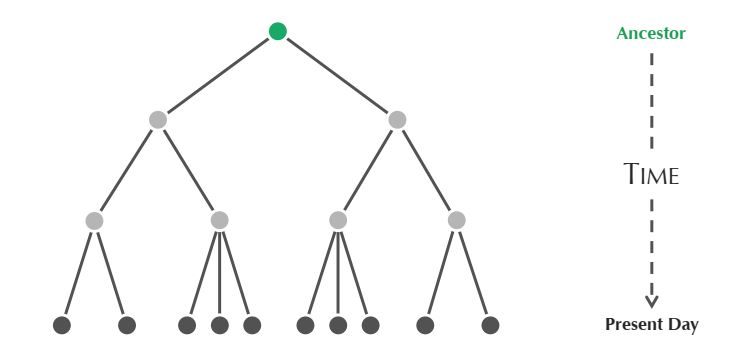
\includegraphics[width=\linewidth]{rooted_tree.jpg}
 	\caption{Albero radicato \cite{bioinfalganactivelearningapproachparttwo}.}
  	\label{fig:RootedTree}
\end{figure}
\newline
\textit{L'albero radicato} si sviluppa a partire da un nodo speciale, chiamato \textit{radice}

\newpage
Ordine dei capitoli:
\begin{itemize}
	\item Cap 3: alberi evolutivi;
	\item Cap 4: albero additivo;
	\item Cap 5: UPGMA (Unweighted Pair Group Method with Arithmetic Mean)
	\item cap 6: NEIGHBORJOINING
\end{itemize}

\begin{center}
\begin{forest}
for tree={circle,draw, l sep=32pt, s sep=33pt}
[k,red 
    [z,edge label={node[midway,left] {5}}
      [y,edge label={node[midway,left] {10}} ] 
      [l,edge label={node[midway,left] {12}}] 
      [m,edge label={node[midway,right] {7}}]
    ]
    [u,edge label={node[midway,right] {2}}
      [f,edge label={node[midway,left] {1}}] 
      [h,edge label={node[midway,left] {18}}] 
      [p,edge label={node[midway,right] {20}}]
  ] 
]
\end{forest}
%\label{fig:phyltree}
\end{center}


\begin{thebibliography}{50}

\bibitem{laBiologiaStrutturaleInMovimento}
Allegretti M. (2014).\newline
\textit{La biologia strutturale in movimento}. \newline
AIRInforma: AIRIcerca.
\\\texttt{\url{http://informa.airicerca.org/it/2014/10/04/biologia-strutturale-in-movimento/}}

\bibitem{SystemsBiologyTheNextFrontierforBioinformatics}
Bacic, A., Likić, V. A., Lithgow, T., McConville, M. J.(2010).\newline 
\textit{Systems Biology: The Next Frontier for Bioinformatics}.\newline
Advances in Bioinformatics, 2010, 1–10. \newline
DOI: \\\texttt{\url{l10.1155/2010/268925}}

\bibitem{BioimageinformaticsanewcategoryinBioinformatics}
Bateman, A., Peng, H., Valencia, A., Wren, J. D. (2012).\newline
\textit{Bioimage informatics: a new category in Bioinformatics}. \newline
Bioinformatics, 28(8), 1057–1057. \newline
DOI: \\\texttt{\url{10.1093/bioinformatics/bts111}}

\bibitem{clinicalApplicationOfBioinformatics}
Bayat Ardeshir (2002).\newline
\textit{Science, medicine, and the future: Bioinformatics}.\newline
BMJ, 324(7344), 1018–1022.
DOI: \\\texttt{\url{10.1136/bmj.324.7344.1018}}

\bibitem{BLAST}
Basic Local Alignment Search Tool Website.\newline
\textit{BLAST}.
\\\texttt{\url{https://blast.ncbi.nlm.nih.gov/Blast.cgi}}

\bibitem{buildingaphylogenictree}
Bear R., Herren C., Horne E., Rintoul D., Smith-Caldas M., Snyder B. \newline
\textit{Building a phylogenetic tree}.
\\\texttt{\url{https://www.khanacademy.org/science/biology/her/tree-of-life/a/building-an-evolutionary-tree}}

\bibitem{BiologySolomon}
Berg L., Martin W. D., Solomon E. \newline
\textit{Biology}.\newline
Brooks Cole, 2010.

\bibitem{MolecularCellBiology}
Berk A., Darnell J., Kaiser A. C., Krieger M., Lodish H., Matsudaira P., Scott P. M., Zipursky L., . \newline
\textit{Molecular Cell Biology}.\newline
W. H. Freeman (2008).

\bibitem{xinformatics}
Borne, K.~D.\newline
\textit{X-Informatics: Practical Semantic Science}.
\\\texttt{\url{http://adsabs.harvard.edu/abs/2009AGUFMIN43E..01B}}. \newline
George Mason University Fairfax VA, American Geophysical Union Fall Meeting, 12/2009.

\bibitem{WhatissystemsbiologyFrontiersinPhysiology}
Breitling, R. (2010). \newline
\textit{What is systems biology? Frontiers in Physiology}.\newline
DOI: \\\texttt{\url{10.3389/fphys.2010.00009}}

\bibitem{campbellBiology}
Cain M., Minorsky P., Reece J, Urry L., Wasserman S. \newline
\textit{Campbell biology}. \newline
Pearson Higher Education, 2016.


\bibitem{computationalApproachForProteinStructurePrediction}
Candavelou, M., Gollapalli, S., Gopal,J., Karthikeyan, K., Venkatesan, A.(2013).\newline \textit{Computational Approach for Protein Structure Prediction}.\newline
Healthcare Informatics Research, 19(2), 137. \newline
DOI: \\\texttt{\url{10.4258/hir.2013.19.2.137}}

\bibitem{bioinfomaticsdefcan}
Can T. (2013).\newline
\textit{Introduction to Bioinformatics}.\newline
miRNomics: MicroRNA Biology and Computational Analysis.\newline
DOI: \\\texttt{\url{10.1007/978-1-62703-748-8_4}}

\bibitem{Abriefhistoryofbioinformatics}
Charette, S. J., Derome, N., Gauthier, J., Vincent, A. T.(2018). \newline
\textit{A brief history of bioinformatics}. \newline
Briefings in Bioinformatics.\newline
DOI: \\\texttt{\url{10.1093/bib/bby063}}

\bibitem{BiologicalDatabaseModeling}
Chen J., Sidhu S. A.\newline
\textit{Biological Database Modeling}.\newline
Norwood, MA, Artech House, 2008.

\bibitem{bioinfalganactivelearningapproachparttwo}
Compeau P., Pevzner P. \newline
\textit{Bioinformatics Algorithms, An Active Learning Approach, Vol II}. \newline
United States Of America, Active Learning Publishers, 2015.

\bibitem{dataMiningInBioinformatics}
Dennis E. Shasha, Hannu Toivonen, Jason T. L. Wang, Mohammed J. Zaki. \newline
\textit{Data Mining in Bioinformatics}.\newline
London, Springer, 2004.

\bibitem{phylogeneticsAnIntroduction}
Emery L.\newline
\textit{Phylogenetics: An introduction}.\newline
European Bioinformatics Institute-European Molecular Biology Laboratory.
\\\texttt{\url{https://www.ebi.ac.uk/training/online/course/introduction-phylogenetics}}\newline
Oxford.

\bibitem{ensembl}
Ensembl Website.\newline
\textit{Ensembl}.
\\\texttt{\url{http://www.ensembl.org/}}

\bibitem{PhylogenetictreesGlasgow}
Gilbert D. \newline
\textit{Phylogenetic trees}.\newline
University of Glasgow, Department of Computing Science.
\\\texttt{\url{http://people.brunel.ac.uk/~csstdrg/courses/glasgow_courses/website_bioinformaticsHM/slides/phylo.pdf}}

\bibitem{phylogenetics}
Haque Sultan Omar (2016).\newline
\textit{Phylogenetics}.\newline
Enciclopedia Britannica.
\\\texttt{\url{https://www.britannica.com/science/phylogenetics\#accordion-article-history}}

\bibitem{icarcnribioinfdefinition} 
ICAR CNR: Istituto Di Calcolo E Reti Ad Alte Prestazioni.\newline
\textit{Bioinformatica}.
\\\texttt{\url{https://www.icar.cnr.it/bio-informatica/}}

\bibitem{sequenceClusteringInBioinformaticsAnEmpiricalStudy}
Jiang, X., Lin, G., Liu, X., Zeng, X., Zou, Q.(2018).\newline
\textit{Sequence clustering in bioinformatics: an empirical study}.\newline
Briefings in Bioinformatics.\newline
DOI: \\\texttt{\url{https://doi.org/10.1093/bib/bby090}}

\bibitem{introductionbioinfalg} 
Jones C. Neil and Pevzner A. Pavel.\newline
\textit{An introduction to bioinformatics algorithms}.\newline
Massachusetts, Massachusetts Institute of Technology, 2004.

\bibitem{mathworksWhatIsTheGeneticAlgorithm}
MathWorks.\newline
\textit{What Is the Genetic Algorithm?}
\\\texttt{\url{https://it.mathworks.com/help/gads/what-is-the-genetic-algorithm.html}}

\bibitem{introductionToGeneticAlgorithmsIncludingExampleCode}
Mallawaarachchi V (2017).\newline
\textit{Introduction To Genetic Algorithms-Including Example Code}.
\\\texttt{\url{https://towardsdatascience.com/introduction-to-genetic-algorithms-including-example-code-e396e98d8bf3}}

\bibitem{bioinformaticsSequenceAndGenomeAnalysis}
Mount W. David.\newline
\textit{Bioinformatics: Sequence and Genome Analysis}.\newline
Cold Spring Harbor Laboratory Press, 2004.

\bibitem{dnaSequencingFactSheet}
National Human Genome Research Institute (2015).\newline
\textit{DNA Sequencing Fact Sheet}.
\\\texttt{\url{https://www.genome.gov/about-genomics/fact-sheets/DNA-Sequencing-Fact-Sheet}}

\bibitem{NCBI}
National Center for Biotechnology Information Website.\newline
\textit{NCBI}.
\\\texttt{\url{https://www.ncbi.nlm.nih.gov/}}

\bibitem{algoritmiEStruttureDati2}
Olivieri M., Verri M. C.\newline
\textit{Algoritmi E Strutture Dati II}.\newline
Dispense, Anno Accademico 2013/2014.

\bibitem{proteineDataBank}
Proteine Data Bank Website.\newline
\textit{PDB}.
\\\texttt{\url{http://www.rcsb.org/}}

\bibitem{bioinformaticsTrendsInGeneExpressionAnalysis}
Raut, A., Raut, S. A., Sathe, S. R.(2010). \newline
\textit{Bioinformatics: Trends in gene expression analysis}.\newline
International Conference on Bioinformatics and Biomedical Technology.\newline
DOI:\\\texttt{\url{10.1109/icbbt.2010.5479003}}

\bibitem{SBW}
Systems Biology Workbench Website.\newline
\textit{SBW}.
\\\texttt{\url{http://sbw.sourceforge.net/}}

\bibitem{phylogeneticsOxford}
Semple C., Steel M.\newline
\textit{Phylogenetics}.\newline
Oxford, Oxford University Press, 2003.

\bibitem{SBML}
Systems Biology Markup Language.\newline
\textit{SBML}.
\\\texttt{\url{http://sbml.org/}}

\bibitem{populationGeneticsAndMicroevolutionaryTheory}
Templeton R. Alan.\newline
\textit{Population Genetics and Microevolutionary Theory}.\newline
Washington University, St. Louis, Missouri, Wiley-Liss, 2006.

\bibitem{treccanibioinf} 
Tramontano Anna (2003).\newline
\textit{La grande scienza. Bioinformatica}.
\\\texttt{\url{http://www.treccani.it/enciclopedia/la-grande-scienza-bioinformatica_\%28Storia-della-Scienza\%29/}}

\end{thebibliography}


%--------------------------------------------------------------
\end{document}
%--------------------------------------------------------------